\chapter{Vorstellung der Abteilung}\index{chp\_Vorstellung_der_Abteilung}

Die Siemens AG ist ein in vielen verschiedenen Bereichen aufgestelltes Technologieunternehmen welches sich  in die in Abbildung \ref*{KernSiemens} dargestellten Kerngeschäftsbereiche unterteilen lässt. Neben an der Börse gelistete ausgegliederte Unternehmen wie Siemens Healthiness, Beschäftigt sich das Unternehmen mit Themen wie Smart infrastructure,  Mobility und Digital Industries. Daneben gibt es noch einen interne und externen Consultingarm mit der Siemens Advanta. Weiterhin gibt es die Portfolio Companies, die Branchenspezifisches Wissen bündeln und im Lösungsgeschäft tätig sind. \cite*{SiemensKern} \\
\begin{figure}[!ht]
    \centering
    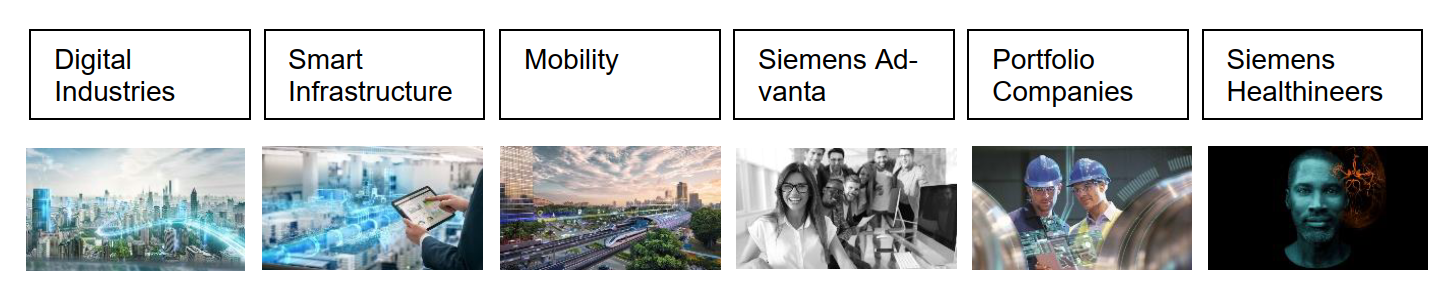
\includegraphics[width=\textwidth]{Pictures/KernSiemens.png}
    \caption{Kerngeschäftsbereiche der Siemens AG}
    \label{KernSiemens}    
\end{figure} \\
Die Unterabteilung Digital Industries (DI) befasst sich mit der Automatisierung und Digitalisierung der diskreten Industrie und der Prozessindustrie.
Die speziellen Branchen, in denen die Digital Industries ihre Produkte und Lösungen vertreibt sind in Abbildung \ref*{DIBranches} dargestellt. \\
\\
\begin{figure}[!ht]
    \centering
    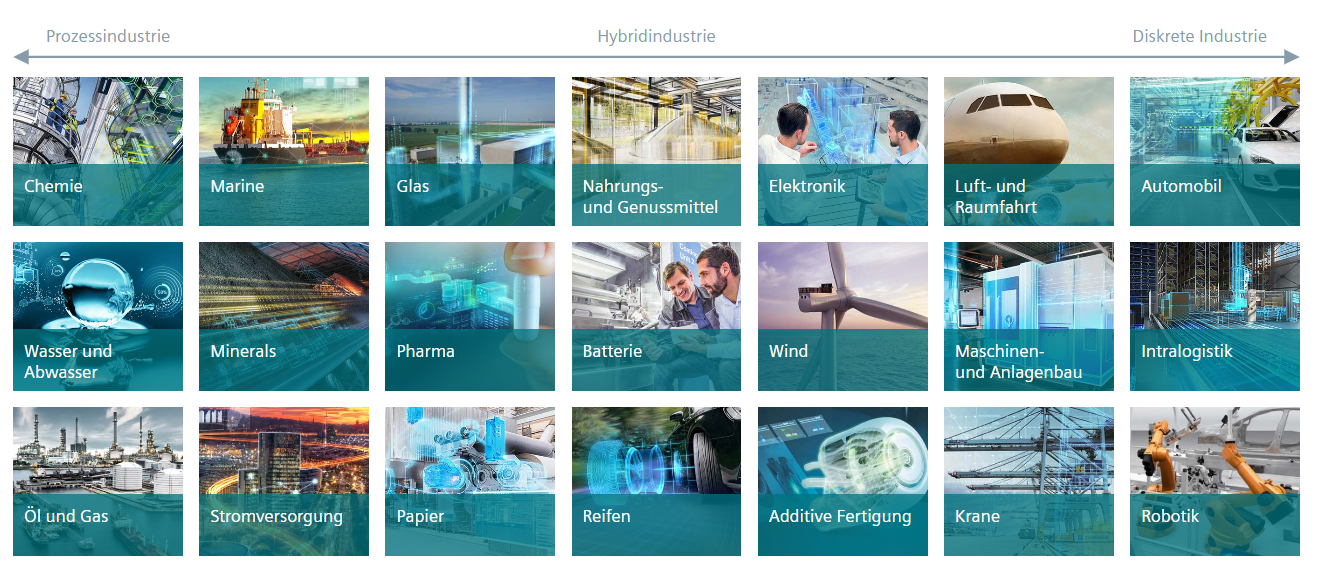
\includegraphics[width=\textwidth]{Pictures/DIBranches.png}
    \caption{Branchen in denen Digital Industries tätig ist}
    \label{DIBranches}    
\end{figure}
In vielen dieser Branchen ist es unabdingbar bei der aktuellen Transformation am Markt, hin zu Industrie 4.0, sämtliche generierten Daten und Steuerungen für die Anlagen und Maschinen digital erreichbar zu halten. \\
Um diesen Bereich abzudecken bietet die Siemens AG die SCALANCE Produktfamilie an: \\
SCALANCE-Geräte bilden die Basis für Kommunikationsnetzwerke in der Fertigungs- und Prozessautomatisierung. Machen Sie Ihre industriellen Netzwerke fit für die Zukunft! Die SCALANCE-Produkte sind speziell für den Einsatz in Industrieanwendungen konzipiert. Damit erfüllen sie alle Voraussetzungen für äußerst effiziente industrielle Netzwerke und Bussysteme. Egal ob Switching, Routing, Security-Anwendungen, Fernzugriff oder Industrial Wireless LAN. \cite*{SCALANCE} \\
In der Abteilung selbst wird die Firmwareentwicklung für die SCALANCE W(WirelessLan) sowie M(Mobilfunk) betrieben. \\
Mit SCALANCE M Mobilfunk-Routern können sowohl ortsfeste Stationen als auch mobile Teilnehmer an eine zentrale Überwachungs- und Steuerungsanlage angeschlossen werden – mit 3G (UMTS), 4G (LTE) oder 5G. \cite*{SCALANCEM}\\
Um den Unternehmen die bestmögliche Infrastruktur für den Austausch von Daten aller Art zu bieten, hat Siemens besondere Industrial Wireless LAN (IWLAN)-Produkte mit speziellen Zusatzfunktionen entwickelt – für die spezifischen Ansprüche von Wi-Fi in der Industrie, im Schaltschrank, Innenbereich sowie Outdoor. Anwendungen in allen Industriebereichen, aber insbesondere in der Automatisierung, wie z. B. der Automobilherstellung, bei Transport und Logistik, aber auch in der Öl- und Gasindustrie profitieren davon. \cite*{SCALANCEW}\\


